\documentclass[aps,pra,notitlepage,amsmath,amssymb,letterpaper,12pt]{revtex4-1}
\usepackage{amsthm}
\usepackage{graphicx}
%  Above uses the Americal Physical Society template for Physical Review A
%  as a reasonable and fully-featured default template
 
%  Below define helpful commands to set up problem environments easily
\newenvironment{problem}[2][Problem]{\begin{trivlist}
\item[\hskip \labelsep {\bfseries #1}\hskip \labelsep {\bfseries #2.}]}{\end{trivlist}}
\newenvironment{solution}{\begin{proof}[Solution]}{\end{proof}}
 
% --------------------------------------------------------------
%                   Document Begins Here
% --------------------------------------------------------------

% In what follows, you can easily change text to see what happens to the document
% For example, replacing the text "Document X" inside the "\title{}" command will
% change the document title
 
\begin{document}
 
\title{Double Well Potential}
\author{Gabriella Nutt}
\affiliation{PHYS 220, Schmid College of Science and Technology, Chapman University}
\date{\today}

\maketitle

\section{Double Well Potential} % Specify main sections this way

% x.yz is the problem number
\begin{problem}{1} 
Consider a ball of mass $m$ with horizontal coordinate $x$ rolling in a double-well potential $V(x) = x^4/4 - x^2/2$. (This is sometimes called the "sombrero" potential. Plot it to see why, for $x\in[-1.5,1.5]$.) This potential produces a force $f_{\text{hat}}(x) = -V'(x) = -x^3 + x$ on the rolling ball. Suppose the ball also has slight friction, so experiences a drag force $f_{\text{drag}}(\dot{x}) = -\nu \dot{x}$. With these forces we thus expect the ball to roll down the sides of the sombrero potential and settle in one of the two stable wells. However, this is boring, so instead we are going to shake the hat back and force periodically with a driving force $f_{\text{drive}}(t) = F\cos(\omega t)$. For small driving forces $F$, this should simply jiggle the ball back and forth at the bottom of one of the stable wells. Our task will be to explore what happens for larger driving forces $F$.
Note that according to Newton's second law, the ball must satisfy the equation of motion: $$m\ddot{x} = f_{\text{hat}}(x) + f_{\text{drag}}(\dot{x}) + f_{\text{drive}}(t) = x - x^3 - \nu \dot{x} + F\cos(\omega t)$$ This system is known as a periodically driven nonlinear "Duffing oscillator," and can be split into a set of two coupled first-order ODEs: $$\dot{x}(t) = y(t)$$ $$m\dot{y}(t) = -\nu y(t) + x(t) - x^3(t) + F\cos(\omega t)$$ Your task will be to solve these equations numerically, for $m=1$, $\nu = 0.25$, and $\omega = 1$. Use a time-step size of $\Delta t = 0.001$ with the 4th-order Runge-Kutta integration method to keep sufficient numerical precision. Implement your code in a python file sombrero.py with suitable test functions in testsombrero.py.
\end{problem}
 
\begin{solution} %You can also use proof in place of solution
In this we solved the differential equations above and observed their behavior on different graphs as their we change the values of F, x(0), and y(0).
From look at all of these graphs it can be found that changing the initial conditions drastically change the behavior. At first it seems like when you change the conditions that the oscillating motion becomes more inconsistent. To further explore the behavior we can strobe the graph at different instances and turn it into a gif. This gives us better insight into the motion of a point. It's very fun. When doing this you actually find the oscillating motion isn't as inconsistent as as it seems when you only observe one moment.
% Use align environments for equations. The \\ is a newline character. The & is the alignment character.
% Using align* or \nonumber on each line removes equation numbers
\end{solution}

\subsection{Here is a scatter plot!} % Specify subsections and subsubsections this way

Figures can be included easily.

\begin{figure}[h!] % h forces the figure to be placed here, in the text
  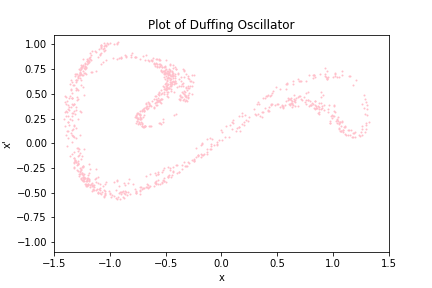
\includegraphics[width=0.4\textwidth]{frame99.png}  % if pdflatex is used, jpg, pdf, and png are permitted
  \caption{Strobe of duffing oscillator.}
  \label{fig:figlabel}
\end{figure}

This text should be below the figure unless \LaTeX  decides that a different layout works better.
 
% Repeat as needed
 
\end{document}
